\documentclass{article}
%\documentclass[utf8]{ctexart}
\usepackage{color}
\usepackage{amsmath}
\usepackage{listings}
\usepackage{graphicx}
\usepackage{biblatex}

\author{cyf, whz}
\title{GHC Compiler Pipeline}

\addbibresource{GHCRef.bib}
\lstset{language=haskell,frame=single}

\begin{document}

	\maketitle
	\paragraph{}
	GHC is structured into two parts:
	\begin{itemize}
		\item The ghc package (in subdirectory \textcolor{red}{compiler}), which implements almost all GHC's functionality. It is an ordinary Haskell library, and can be imported into a Haskell program by \textcolor{cyan}{import GHC}.
		\item The ghc binary (in subdirectory \textcolor{red}{ghc}) which imports the ghc package, and implements the I/O for the ghci interactive loop.
	\end{itemize}
	\paragraph{}
	GHC is the root module for the GHC API, with very little code and just simple wrappers.
	\paragraph{}
	GhcMake implements \textcolor{magenta}{--make} and deals with compiling multiple modules.
	\paragraph{}
	DriverPipeline, after GhcMake, deals with compiling a single module through all its stages, including cpp, unlit, compile, assemble, link, etc. These stages/phases call other program and generate a series of intermediate files. The driver pipeline is not the same thing as compilation pipeline and the latter is part of the former.
	\paragraph{}
	When compile \textcolor{red}{Foo.hs} or \textcolor{red}{Foo.lhs} (Literate Haskell), the following phases are called (actually depend on file extensions or flags):
	\begin{itemize}
		\item The \textbf{unlit pre-processor} \textcolor{cyan}{unlit}, which locates at \textcolor{red}{utils/unlit} as C program, removes the literate markup and generates \textcolor{red}{Foo.lpp}.
		\item The \textbf{C preprocessor} \textcolor{cyan}{cpp} (when \textcolor{magenta}{-cpp} is specified), generates \textcolor{red}{Foo.hspp}
		\item The \textbf{compiler}, which does not start a separate process, generates files according to the flag given by user.
	\end{itemize}
	\begin{lstlisting}
bash$ ghc -c Foo.hs -O -dshow-passes
*** Parser:
*** Renamer/typechecker:
*** Desugar:
Result size of Desugar (after optimization)
  = {terms: 7, types: 4, coercions: 0}
*** Simplifier:
Result size of Simplifier iteration=1
  = {terms: 6, types: 3, coercions: 0}
Result size of Simplifier = {terms: 6, types: 3, coercions: 0}
*** Specialise:
Result size of Specialise = {terms: 6, types: 3, coercions: 0}
*** Float out(FOS {Lam = Just 0, Consts = True, PAPs = False}):
Result size of Float out(FOS {Lam = Just 0,Consts = True,PAPs = False})
  = {terms: 8, types: 4, coercions: 0}
*** Float inwards:
Result size of Float inwards = {terms: 8, types: 4, coercions: 0}
*** Simplifier:
Result size of Simplifier iteration=1
  = {terms: 12, types: 6, coercions: 0}
Result size of Simplifier = {terms: 9, types: 5, coercions: 0}
*** Simplifier:
Result size of Simplifier = {terms: 9, types: 5, coercions: 0}
*** Simplifier:
Result size of Simplifier = {terms: 9, types: 5, coercions: 0}
*** Demand analysis:
Result size of Demand analysis = {terms: 9, types: 5, coercions: 0}
*** Worker Wrapper binds:
Result size of Worker Wrapper binds
  = {terms: 9, types: 5, coercions: 0}
*** Simplifier:
Result size of Simplifier = {terms: 9, types: 5, coercions: 0}
*** Float out(FOS {Lam = Just 0, Consts = True, PAPs = True}):
Result size of Float out(FOS {Lam = Just 0,Consts = True, PAPs = True})
  = {terms: 9, types: 5, coercions: 0}
*** Common sub-expression:
Result size of Common sub-expression
  = {terms: 9, types: 5, coercions: 0}
*** Float inwards:
Result size of Float inwards = {terms: 9, types: 5, coercions: 0}
*** Simplifier:
Result size of Simplifier = {terms: 9, types: 5, coercions: 0}
*** Tidy Core:
Result size of Tidy Core = {terms: 9, types: 5, coercions: 0}
*** CorePrep:
Result size of CorePrep = {terms: 12, types: 6, coercions: 0}
*** Stg2Stg:
*** CodeOutput:
*** New CodeGen:
	\end{lstlisting}
	\paragraph{}
	\textcolor{red}{HscMain} is used in compile phase of driver pipeline. It compiles a single module/expression/statement to bytecode/M.hc/M.s file. It is also called by GHCi.
	\paragraph{}
	GHC supports three backend code generators currently:
	\begin{itemize}
		\item native code generator
		\item C code generator
		\item llvm code generator
	\end{itemize}
	\paragraph{}
	And the possible range of outputs depends on the backend used, all three support assembly output.
	\begin{itemize}
		\item \textbf{Object code} \textcolor{red}{Foo.o}: no flags required
		\item \textbf{Assembly code} \textcolor{red}{Foo.s}: \textcolor{magenta}{-S} required
		\item \textbf{C code}: \textcolor{magenta}{-C} required
	\end{itemize}
	\paragraph{}
	The first two ways are supported by three backend and the last one is only supported by C backend.
	\paragraph{}
	Pipeline of \textcolor{red}{compiler/main/HscMain.hs} is following. They can be dumped by flags like \textcolor{magenta}{-ddump-*}
	\begin{itemize}
		\item The \textbf{Front End} processes the program in the big \textcolor{red}{HsSyn} type, which is parameterised over the types of the term variables it contains. These three passes detects all programmer errors, and sort them and report them to the user.
		\begin{itemize}
			\item The \textbf{Parser} produces \textcolor{red}{HsSyn} parameterised by \textcolor{red}{RdrName}, which is approximately a string. (\textcolor{magenta}{-ddump-parsed})
			\item The \textbf{Renamer} transforms \textcolor{red}{HsSyn} such that it is parameterised by \textcolor{red}{Name}, which is approximately a string plus a \textcolor{red}{Unique} (number) that uniquely identifies it. (\textcolor{magenta}{ddump-rn})
			\item The \textbf{Typechecker} performs type reconstruction and further transforms \textcolor{red}{HsSyn} such that it is parameterised by \textcolor{red}{Id}, which is approximately a \textcolor{red}{Name} plus a type.
		\end{itemize}
		\item The \textbf{Desugarer} (\textcolor{red}{compiler/deSugar/Desugar.hs}) converts the massive \textcolor{red}{HsSyn} to GHC's intermediate language \textcolor{red}{CoreSyn}, which is concise and amazing expressive power. It is much more common to desugar the program before typechecking or renaming, because that presents the renamer and typechecker with a much smaller language to deal with. However, GHC's organisation intend to display precisely error massages for users and avoid preserving type-inference properties.
	\end{itemize}
	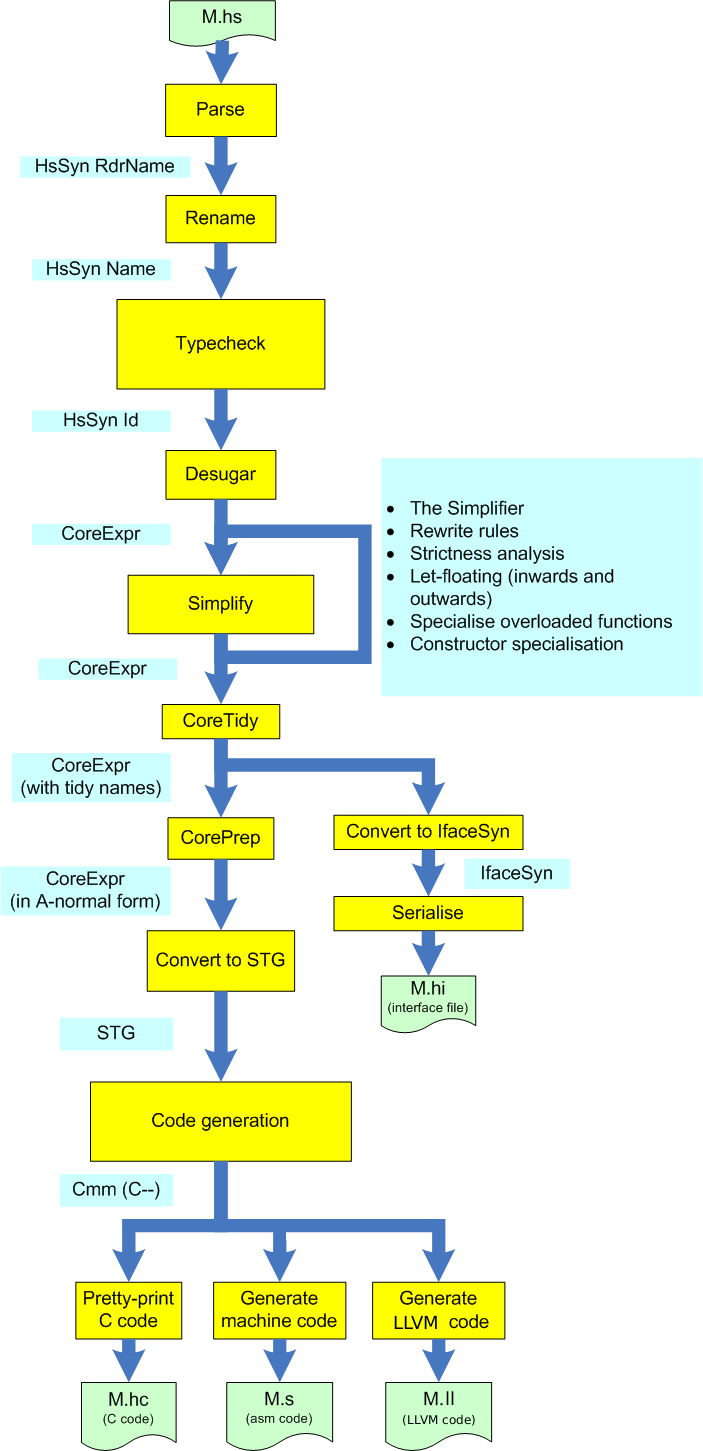
\includegraphics[width=4.57in,height=7.5in]{HscPipe2.png}
	\paragraph{}
	\begin{itemize}
		\item The \textcolor{red}{SimplCore} pass (\textcolor{red}{compiler/simplCore/SimplCore.hs}) is a bunch of Core-to-Core passes that optimise the program.
		\begin{itemize}
			\item The Simplifier
			\begin{itemize}
				\item Inlining
				\item Rewrite rules
				\item Beta reduction
				\item Case of case
				\item Case of known constructor
				\item etc etc etc...
			\end{itemize}
			\item Specialise overloading
			\item Float out
			\item Float in
			\item Demand, cardinality, and CPR analysis
			\item Arity analysis
			\item Call-pattern specialisation (SpecConstr)
		\end{itemize}
		The simplifier implements and applies lots of small, local optimisations to the program, making them cascade nicely. The float-out and float-in transformations move let-bindings outwards and inwards to optimise the program.
		\item The \textbf{CoreTidy} pass gets the code into a form in which it can be imported into subsequent modules.
		\item The \textbf{CorePrep} pass is the first step of feeding the tidied Core program to the Back End. Here a Core-to-Core pass puts the program into A-normal form (ANF).
		\item The \textbf{CoreToStg} pass is the second step to produce \textcolor{red}{StgSyn} data type.
		\item The \textbf{Code generator} converts the STG program to a \textcolor{cyan}{c--} program.
	\end{itemize}
\end{document}



